\documentclass[11pt]{article}
\usepackage[T1]{fontenc}
\usepackage{lmodern}
\usepackage[letterpaper,margin=1in]{geometry}
\usepackage{amsmath,amssymb,amsthm,mathtools}
\usepackage{microtype}
\usepackage{booktabs,array}
\usepackage{xcolor}
\usepackage{tikz}
\usepackage{caption}
\usepackage{xurl}
\usepackage[colorlinks=true,linkcolor=blue!45!black,citecolor=blue!45!black,urlcolor=blue!45!black]{hyperref}
\hypersetup{pdftitle={A computer-assisted proof of the optimal packing of six equilateral triangles},pdfauthor={Kevin M. Neal},pdfsubject={Exact geometric packing, finite certificates, computer-assisted proof},pdfkeywords={equilateral triangles, packing, computer-assisted proof, exact certificate}}
\newtheorem{theorem}{Theorem}[section]
\newtheorem{lemma}[theorem]{Lemma}
\newtheorem{corollary}[theorem]{Corollary}
\captionsetup{font=small,labelfont=bf}
\setlength{\emergencystretch}{2em}
\setlength{\parskip}{3pt}
\setlength{\tabcolsep}{5pt}
\allowdisplaybreaks[1]
\title{A computer-assisted proof of the optimal packing\\of six equilateral triangles}
\author{Kevin M. Neal\\[3pt]\footnotesize\href{https://orcid.org/0000-0003-4360-8027}{ORCID: 0000-0003-4360-8027}}
\date{Preprint v1.0.0 --- 8 October 2026}
\begin{document}
\maketitle
\begin{abstract}
We give an exact computer-assisted proof that the least side length of an equilateral triangle containing six unit equilateral triangles with pairwise disjoint interiors is $(13+3\sqrt{13})/8$. The six triangles may rotate independently, and boundary contact is allowed. An analytic replacement theorem reduces the problem to packing three arbitrary unit triangles in a clipped hexagon. A rational, closed-domain certificate then excludes every normalized configuration except neighborhoods of an exact construction. A separate local theorem identifies every target-side feasible configuration in those neighborhoods. Its proof combines complete separating-axis branches, uniform derivative bounds, and nonnegative dual identities over $\mathbb Q(\sqrt3,\sqrt{13})$. The global certificate has 22,329 outer nodes and no unresolved leaves. Its acceptance uses exact rational and algebraic arithmetic, without numerical optimization or floating-point sign decisions. We give the analytic reductions, the certificate rules, and the trust boundary of the computation; the result is not a proof-kernel formalization.
\end{abstract}

\section{Statement and structure of the proof}\label{sec:statement}

A packing means a collection of closed triangles whose two-dimensional interiors are pairwise disjoint. Their boundaries may meet. Let $s(6)$ be the infimum of the side lengths of equilateral triangles containing six equilateral triangles of side one. Translations and rotations of the six pieces are independent.

\begin{theorem}\label{thm:main}
The minimum is attained and
\[
 s(6)=T:=\frac{13+3\sqrt{13}}8
       =2.9770817282989959849\ldots.
\]
\end{theorem}

The upper bound is an explicit algebraic construction. The lower bound has two analytic reductions and one finite computational premise. First, a corner-capacity argument permits the simultaneous replacement of up to three pieces by the aligned unit triangles at the container's corners. Three original pieces survive unchanged. They lie in a hexagon $H(S)$ defined below. Second, a local rigidity theorem at side $T$ identifies the three surviving pieces whenever their poses are sufficiently close to a specified reference triple. Between these reductions, an exact finite certificate covers the entire normalized three-piece domain. Every terminal is either an exclusion or an application of the local theorem.

The local statement fixes two corner pieces and the container exactly. It does not isolate every pose in the six-piece construction: the third corner piece is unnecessary to that statement, and the six-piece witness has a rattler. The proof also does not classify all optimal packings before corner replacement. No full-side contact, lozenge, common orientation, or prescribed contact graph is assumed in the global problem.

Friedman's packing catalogue attributes the attaining construction to Maurizio Morandi, August 2008~\cite{FriedmanTrianglesInTriangles}. Chou's manuscript dated January 2016 explicitly recorded the six-piece value as found but not proved~\cite{Chou2016}. The present work concerns its unrestricted lower bound and an exact finite certificate, not discovery of a new construction. A bounded literature search completed on 8 October 2026 did not locate an earlier published optimality proof; that search is not a claim about all unpublished or unindexed work.

Related triangle covering questions require different hypotheses. For example, Baek and Lee's covering theorem concerns triangles with parallel sides, while their Question~19 separately asks about finite congruent triangle packings~\cite{BaekLee2025}. Covering permits overlaps and need not impose containment of each covering piece; it does not provide the lower bound needed here. Likewise, general triangle-packing complexity results with varying input sizes or piece sizes do not resolve this fixed six-congruent-piece instance.

\begin{figure}[htbp]
\centering
\begin{minipage}{0.46\textwidth}\centering
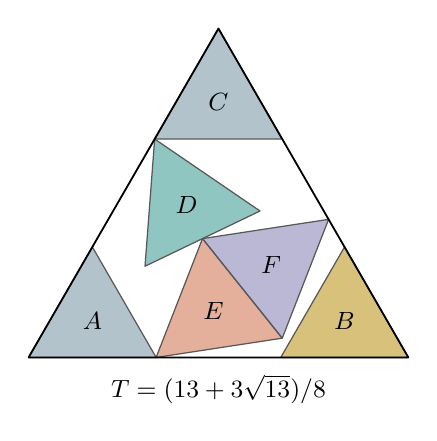
\begin{tikzpicture}[x=1.62cm,y=1.62cm,line join=round]
\definecolor{pieceA}{HTML}{6d8c9b}
\filldraw[fill=pieceA,fill opacity=0.52,draw=black!65,line width=.45pt] (0.000000000,0.000000000) -- (1.000000000,0.000000000) -- (0.500000000,0.866025404) -- cycle;
\node[font=\small] at (0.500000000,0.288675135) {$ A $};
\definecolor{pieceB}{HTML}{b58900}
\filldraw[fill=pieceB,fill opacity=0.52,draw=black!65,line width=.45pt] (1.977081728,0.000000000) -- (2.977081728,0.000000000) -- (2.477081728,0.866025404) -- cycle;
\node[font=\small] at (2.477081728,0.288675135) {$ B $};
\definecolor{pieceC}{HTML}{6d8c9b}
\filldraw[fill=pieceC,fill opacity=0.52,draw=black!65,line width=.45pt] (0.988540864,1.712203002) -- (1.988540864,1.712203002) -- (1.488540864,2.578228406) -- cycle;
\node[font=\small] at (1.488540864,2.000878137) {$ C $};
\definecolor{pieceD}{HTML}{2a9188}
\filldraw[fill=pieceD,fill opacity=0.52,draw=black!65,line width=.45pt] (0.912846955,0.715071901) -- (1.814234774,1.148084603) -- (0.988540864,1.712203002) -- cycle;
\node[font=\small] at (1.238540864,1.191786502) {$ D $};
\definecolor{pieceE}{HTML}{cb6640}
\filldraw[fill=pieceE,fill opacity=0.52,draw=black!65,line width=.45pt] (1.000000000,0.000000000) -- (1.988540864,0.150953502) -- (1.363540864,0.931578252) -- cycle;
\node[font=\small] at (1.450693909,0.360843918) {$ E $};
\definecolor{pieceF}{HTML}{7b77ad}
\filldraw[fill=pieceF,fill opacity=0.52,draw=black!65,line width=.45pt] (1.363540864,0.931578252) -- (1.988540864,0.150953502) -- (2.352081728,1.082531755) -- cycle;
\node[font=\small] at (1.901387819,0.721687836) {$ F $};
\draw[line width=.65pt] (0.000000000,0.000000000) -- (2.977081728,0.000000000) -- (1.488540864,2.578228406) -- cycle;
\node[below,font=\small] at (1.488540864,-.06) {$T=(13+3\sqrt{13})/8$};
\end{tikzpicture}\par\smallskip
(a) Attaining construction.
\end{minipage}\hfill
\begin{minipage}{0.46\textwidth}\centering
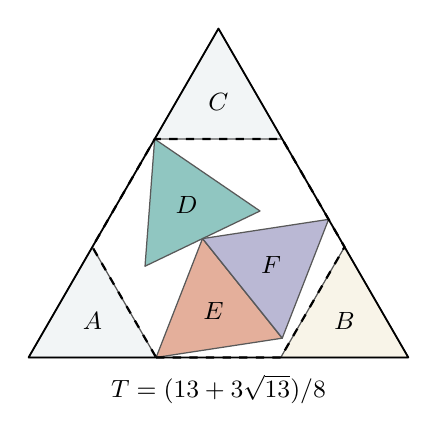
\begin{tikzpicture}[x=1.62cm,y=1.62cm,line join=round]
\definecolor{pieceA}{HTML}{6d8c9b}
\filldraw[fill=pieceA,fill opacity=0.09,draw=black!65,line width=.45pt] (0.000000000,0.000000000) -- (1.000000000,0.000000000) -- (0.500000000,0.866025404) -- cycle;
\node[font=\small] at (0.500000000,0.288675135) {$ A $};
\definecolor{pieceB}{HTML}{b58900}
\filldraw[fill=pieceB,fill opacity=0.09,draw=black!65,line width=.45pt] (1.977081728,0.000000000) -- (2.977081728,0.000000000) -- (2.477081728,0.866025404) -- cycle;
\node[font=\small] at (2.477081728,0.288675135) {$ B $};
\definecolor{pieceC}{HTML}{6d8c9b}
\filldraw[fill=pieceC,fill opacity=0.09,draw=black!65,line width=.45pt] (0.988540864,1.712203002) -- (1.988540864,1.712203002) -- (1.488540864,2.578228406) -- cycle;
\node[font=\small] at (1.488540864,2.000878137) {$ C $};
\definecolor{pieceD}{HTML}{2a9188}
\filldraw[fill=pieceD,fill opacity=0.52,draw=black!65,line width=.45pt] (0.912846955,0.715071901) -- (1.814234774,1.148084603) -- (0.988540864,1.712203002) -- cycle;
\node[font=\small] at (1.238540864,1.191786502) {$ D $};
\definecolor{pieceE}{HTML}{cb6640}
\filldraw[fill=pieceE,fill opacity=0.52,draw=black!65,line width=.45pt] (1.000000000,0.000000000) -- (1.988540864,0.150953502) -- (1.363540864,0.931578252) -- cycle;
\node[font=\small] at (1.450693909,0.360843918) {$ E $};
\definecolor{pieceF}{HTML}{7b77ad}
\filldraw[fill=pieceF,fill opacity=0.52,draw=black!65,line width=.45pt] (1.363540864,0.931578252) -- (1.988540864,0.150953502) -- (2.352081728,1.082531755) -- cycle;
\node[font=\small] at (1.901387819,0.721687836) {$ F $};
\draw[dashed,line width=.8pt] (1.000000000,0.000000000) -- (1.977081728,0.000000000) -- (2.477081728,0.866025404) -- (1.988540864,1.712203002) -- (0.988540864,1.712203002) -- (0.500000000,0.866025404) -- cycle;
\draw[line width=.65pt] (0.000000000,0.000000000) -- (2.977081728,0.000000000) -- (1.488540864,2.578228406) -- cycle;
\node[below,font=\small] at (1.488540864,-.06) {$T=(13+3\sqrt{13})/8$};
\end{tikzpicture}\par\smallskip
(b) The remaining hexagon $H(T)$.
\end{minipage}
\caption{The exact reference packing, drawn with rounded coordinates. The dashed cuts in (b) remove the three aligned unit corner interiors. The corner-replacement theorem applies to arbitrary packings; the depicted survivor triple is the reference example, not an assumed contact pattern.}\label{fig:construction}
\end{figure}

\section{Coordinates and the exact construction}\label{sec:upper}

\subsection{Oblique coordinates}

We use the oblique-to-Cartesian map
\[
 \Phi(u,v)=\left(u+\frac v2,\frac{\sqrt3}2v\right),
 \qquad N(u,v)=\|\Phi(u,v)\|^2=u^2+uv+v^2.
\]
The side-$L$ container is
\[
 \Delta_L=\{(u,v):u\ge0,\ v\ge0,\ u+v\le L\}.
\]
All Euclidean distances in oblique coordinates are computed using $N$. Linear functionals in these coordinates are covectors; they need not be Euclidean unit normals.

Put
\[
 Q_0=\operatorname{conv}\left\{
 (-1/3,-1/3),(2/3,-1/3),(-1/3,2/3)\right\},
\quad
 M(c,b)=\begin{pmatrix}c-b&-2b\\2b&c+b\end{pmatrix}.
\]
If $c^2+3b^2=1$, then $M(c,b)$ is the Euclidean rotation with cosine $c$ and sine $\sqrt3 b$, expressed in oblique coordinates. The unit triangle with centroid $p$ and this orientation is $p+M(c,b)Q_0$.

\subsection{Reference poses and exact nonoverlap}

Write $r=\sqrt{13}$ and $h=\sqrt3/2$. The six reference poses are given in Table~\ref{tab:poses}.
\begin{table}[htbp]
\centering
\small
\begin{tabular}{c c c c}
\hline
Piece & Centroid $p$ & $c$ & $b$\\\hline
$A$ & $(1/3,1/3)$ & $1$ & $0$\\
$B$ & $(T-2/3,1/3)$ & $1$ & $0$\\
$C$ & $(1/3,T-2/3)$ & $1$ & $0$\\
$D$ & $((3+r)/12,\,5(3+r)/24)$ & $r/4$ & $1/4$\\
$E$ & $((19+3r)/24,\,5/12)$ & $(5+3r)/16$ & $(5-r)/16$\\
$F$ & $((7+3r)/12,\,5/6)$ & $5/8$ & $-r/8$\\\hline
\end{tabular}
\caption{The exact upper-bound construction.}\label{tab:poses}
\end{table}

For each row, $c^2+3b^2=1$. Table~\ref{tab:vertices} lists the actual oblique vertices. It also fixes the local vertex order used later. For $D$, this order is the cyclic permutation $(2,0,1)$ of the order obtained by applying $M(c,b)$ to the three displayed vertices of $Q_0$. For every other piece, the displayed order agrees with the generated order. All orders are counterclockwise in Cartesian coordinates.

\begin{table}[htbp]
\centering
\small
\begin{tabular}{c c c c}
\hline
 & $v_0$ & $v_1$ & $v_2$\\\hline
$A$ & $(0,0)$ & $(1,0)$ & $(0,1)$\\
$B$ & $(T-1,0)$ & $(T,0)$ & $(T-1,1)$\\
$C$ & $(0,T-1)$ & $(1,T-1)$ & $(0,T)$\\
$D$ & $(0,T-1)$ & $(1/2,(3+r)/8)$ & $((1+r)/4,(7+r)/8)$\\
$E$ & $(1,0)$ & $(1+r/4,(5-r)/8)$ & $((3+r)/8,(5+r)/8)$\\
$F$ & $((3+r)/8,(5+r)/8)$ & $(1+r/4,(5-r)/8)$ & $((3+3r)/8,5/4)$\\\hline
\end{tabular}
\caption{Reference vertices, including the local anchor convention: the anchor of each piece is $v_0$.}\label{tab:vertices}
\end{table}

For a counterclockwise owner triangle $X$ and an edge $e=(v_k,v_{k+1})$, with indices modulo three, define the Cartesian separating gaps against $Y$ by
\begin{equation}\label{eq:gap}
 G_{X,k;Y,\ell}
 =-\det\bigl(\Phi(v_{k+1}-v_k),\Phi(w_\ell-v_k)\bigr),
 \qquad \ell=0,1,2.
\end{equation}
If all three gaps are nonnegative, $Y$ lies in the closed exterior halfplane of that edge, and the interiors of $X,Y$ are disjoint. Table~\ref{tab:separation} gives one such feature for each of the fifteen pairs. The last column is the minimum of the three gaps divided by $h$. Since $r>3$, every entry is nonnegative.

\begin{table}[htbp]
\centering
\small
\begin{tabular}{c c c@{\qquad}c c c}
\hline
Pair & Owner-edge & $\min G/h$ & Pair & Owner-edge & $\min G/h$\\\hline
$AB$ & $A,1$ & $3(r-1)/8$ & $AC$ & $A,1$ & $3(r-1)/8$\\
$AD$ & $A,1$ & $(r-1)/8$ & $AE$ & $A,1$ & $0$\\
$AF$ & $A,1$ & $r/4$ & $BC$ & $B,2$ & $3(r-1)/8$\\
$BD$ & $B,2$ & $(3+r)/8$ & $BE$ & $B,2$ & $(r-3)/8$\\
$BF$ & $B,2$ & $(r-3)/8$ & $CD$ & $C,0$ & $0$\\
$CE$ & $C,0$ & $r/4$ & $CF$ & $C,0$ & $(3r-5)/8$\\
$DE$ & $D,1$ & $0$ & $DF$ & $D,1$ & $0$\\
$EF$ & $E,1$ & $0$ & & &\\\hline
\end{tabular}
\caption{Exact pairwise separation witnesses.}\label{tab:separation}
\end{table}

The vertices in Table~\ref{tab:vertices} satisfy $u,v\ge0$ and $u+v\le T$; these are direct linear comparisons in $\mathbb Q(r)$. Table~\ref{tab:poses} verifies the unit side lengths, and Table~\ref{tab:separation} verifies all pairwise nonoverlap. Thus
\begin{equation}\label{eq:upper}
 s(6)\le T.
\end{equation}
In particular, attainment at the claimed value will follow once the strict lower-bound exclusion is proved.

\section{An analytic corner-replacement theorem}\label{sec:corner}

The reduction in this section is independent of the reference construction.

\subsection{Wedged triangles and their depth}

Let $W=\{u,v\ge0\}$ and $A_0=\operatorname{conv}\{(0,0),(1,0),(0,1)\}$. A unit equilateral triangle in $W$ has an orientation representative $\beta\in[-\pi/3,\pi/3]$. Set
\[
 a=\frac{|\sin\beta|}{\sqrt3},\qquad c=\cos\beta,\qquad q=c+a.
\]
Then $0\le a\le1/2$, $c^2+3a^2=1$, $c\ge1/2$, and $c\ge a$. Moreover
\[
 c^2-(1-a)^2=2a(1-2a)\ge0
\]
with both compared quantities nonnegative, so $q\ge1$.

Translate the triangle so that its minimum $u$ and minimum $v$ are zero. Inspection of the rotated unit vertices gives one of the two forms
\begin{align}\label{eq:wedged}
 J_+&=\operatorname{conv}\{(2a,0),(q,2a),(0,q)\},\\
 J_-&=\operatorname{conv}\{(0,2a),(2a,q),(q,0)\}.\notag
\end{align}
Consequently every unit triangle $J\subset W$ is one of these forms translated by $(x,y)$ with $x,y\ge0$. Since $q\ge2a$, its depth is
\begin{equation}\label{eq:depth}
 d(J):=\min_{p\in J}(p_u+p_v)=2a+x+y.
\end{equation}
Its interior meets the interior of $A_0$ if and only if $d(J)<1$. One direction follows immediately from the defining inequalities of $A_0$. For the converse, a point of $J$ with sum below one is approximated by two-dimensional interior points of $J$. These have positive coordinates, since $J\subset W$, and their sum remains below one.

\subsection{Two support inequalities, with all sign cases}

\begin{lemma}\label{lem:support}
Let $n=(n_u,n_v)$ be a nonzero covector with $M=\max(n_u,n_v)>0$ and $m=\min(n_u,n_v)$. For every unit triangle $J\subset W$,
\begin{equation}\label{eq:support-upper}
 \min_{p\in J}n\cdot p\le M d(J)+\min(0,m).
\end{equation}
For every unit triangle $K\subset W$ with $d(K)\le1$,
\begin{equation}\label{eq:support-lower}
 \max_{p\in K}n\cdot p\ge M+\min(0,m).
\end{equation}
\end{lemma}

\begin{proof}
Divide by $M$ and exchange $u,v$ if necessary. It suffices to consider $n=(1,z)$ with $z\le1$; the exchange interchanges the two forms in \eqref{eq:wedged}. For the upper bound, take vertex $(2a,0)$ of $J_+$ or $(0,2a)$ of $J_-$ when $z\ge0$, and vertex $(0,q)$ of $J_+$ or $(2a,q)$ of $J_-$ when $z<0$. Add $(x,y)$ in each case. For the lower bound, take $(q,2a)$ of $K_+$ or $(q,0)$ of $K_-$, again with the translation.

Table~\ref{tab:eight-cases} gives all eight algebraic differences. In its lower-bound rows, $w=1-2a-x-y\ge0$. In upper-bound rows the difference is the asserted upper bound minus the selected value; in lower-bound rows it is the selected value minus the asserted lower bound. Every displayed summand is nonnegative in its specified range. Direct expansion verifies each identity, proving both inequalities.
\begin{table}[htbp]
\centering
\small
\begin{tabular}{c c c l}
\hline
Bound & Form & Range & Nonnegative difference\\\hline
Upper & $J_+$ & $0\le z\le1$ & $(1-z)y$\\
Upper & $J_-$ & $0\le z\le1$ & $(1-z)(2a+y)$\\
Upper & $J_+$ & $z<0$ & $2a+(1-z)y+(-z)(q-1)$\\
Upper & $J_-$ & $z<0$ & $(1-z)y+(-z)(q-1)$\\
Lower & $K_+$ & $0\le z\le1$ & $(q-1)+2az+x+zy$\\
Lower & $K_-$ & $0\le z\le1$ & $(q-1)+x+zy$\\
Lower & $K_+$ & $z<0$ & $(q-1)+(1-z)x+(-z)w$\\
Lower & $K_-$ & $z<0$ & $(q-1)+(1-z)x+(-z)(2a+w)$\\\hline
\end{tabular}
\caption{Complete support-inequality verification.}\label{tab:eight-cases}
\end{table}
\end{proof}

\begin{lemma}[Corner capacity]\label{lem:corner-capacity}
Two unit equilateral triangles in $W$ whose interiors both meet the interior of $A_0$ cannot have disjoint interiors.
\end{lemma}

\begin{proof}
Otherwise weak separation of the two convex interiors gives a nonzero covector $n$ such that
\[
 \max_{p\in K}n\cdot p\le\min_{p\in J}n\cdot p.
\]
If $\max(n_u,n_v)\le0$, negate $n$ and exchange $J,K$. We may therefore assume $M>0$. Both depths are strictly below one. Lemma~\ref{lem:support} gives
\[
 \min_Jn\cdot p\le Md(J)+\min(0,m)
 <M+\min(0,m)\le\max_Kn\cdot p,
\]
contradicting separation. The strict intrusion of both triangles is used here; replacing either depth hypothesis by an unjustified weak one would invalidate the argument.
\end{proof}

\begin{theorem}[Simultaneous corner replacement]\label{thm:corners}
If $n\ge3$ unit equilateral triangles pack in $\Delta_S$ with $S\ge2$, then $n$ unit equilateral triangles pack there with three pieces equal to its aligned unit corner triangles.
\end{theorem}

\begin{proof}
Apply Lemma~\ref{lem:corner-capacity} in the wedge at each container corner. Each prescribed corner triangle has interior overlap with at most one original piece. Remove the union of the offending pieces, whose cardinality is at most three. Insert all three prescribed corner triangles. They have disjoint interiors for $S\ge2$, and no survivor has interior overlap with any of them. At least $n-3$ original pieces remain. Keep the inserted corners and any $n-3$ survivors, discarding surplus survivors if necessary. The original surviving poses have not moved. The replacement need not be realizable by a continuous motion and does not preserve labels.
\end{proof}

Define the clipped hexagon
\begin{equation}\label{eq:hexagon}
 H(S)=\{0\le u,v\le S-1,\quad1\le u+v\le S\}.
\end{equation}
A triangle in $\Delta_S$ disjoint in interior from all three aligned corner pieces lies in $H(S)$. For the corner at the origin this is the depth condition $u+v\ge1$; the other two corners give $u,v\le S-1$. If a vertex strictly violated one of these cuts, interior approximation would produce interior-interior overlap. Conversely, any triangle in $H(S)$ is interior-disjoint from the three corners.

\begin{corollary}\label{cor:hexagon-reduction}
For $S\ge2$, six unit triangles pack in $\Delta_S$ if and only if three arbitrary unit triangles pack in $H(S)$. In the forward direction, the three surviving triangles can be chosen from the original packing without changing their poses or their original coordinate frame.
\end{corollary}

The area bound for any six-piece packing is $S^2\ge6$, so all candidates relevant to Theorem~\ref{thm:main} satisfy $S>2$. Thus no smaller-side case is lost by the corollary.

\section{A finite exact local theorem}\label{sec:local}

The local theorem is the mechanism by which a closed search can terminate at a feasible reference packing. Excluding an entire neighborhood of that packing at side $T$ would be impossible.

\subsection{Coordinates and necessary branch systems}

Use the reference vertex orders in Table~\ref{tab:vertices}, and work now in Cartesian coordinates. The pose of a variable piece $i$ is
\[
 a_i+R(\phi_i)(v_{i,\ell}^*-v_{i,0}^*),\qquad \ell=0,1,2,
\]
where $a_i$ is its Cartesian anchor, $R$ is the usual rotation matrix, and a star denotes the reference. The local error is $a_i-v_{i,0}^*$ together with the radian angle $\phi_i$. Fix $A,C$ and the side $T$ exactly. Only $D,E,F$ vary, giving nine coordinates. The exceptional coordinate is $\phi_D$; the other eight coordinates are called transverse.

\begin{theorem}[Fixed-corner local isolation]\label{thm:local}
Suppose $A,C,D,E,F$ pack in $\Delta_T$, with $A,C$ fixed exactly as above. If every Cartesian anchor-error component and every radian rotation of $D,E,F$ has absolute value at most $\rho=1/50$, then the three variable pieces have exactly their reference poses.
\end{theorem}

For precise finite definitions, index $A,C,D,E,F$ by $i=0,1,2,3,4$, respectively. Temporarily use coordinates $z_{3i},z_{3i+1},z_{3i+2}$ for Cartesian anchor and angle, and $z_{15}$ for container side. Only indices in
\[
 I=\{6,7,8,9,10,11,12,13,14\}
\]
vary in this theorem; index $8$ is $\phi_D$. Let
\[
 w_0(x,y)=y,\quad w_1(x,y)=\sqrt3x-y,\quad
 w_2(x,y)=\sqrt3(T-x)-y.
\]
Write $W_{ivw}$ for the wall gap $w_w$ of vertex $v$ of piece $i$, and $G_{iejv}$ for the separating gap \eqref{eq:gap} with owner $i$, edge $e$, other piece $j$, and other vertex $v$.

Retain the following eleven zero-reference wall gaps, in the displayed order:
\begin{equation}\label{eq:wall-list}
 W_{000},W_{001},W_{010},W_{021},W_{101},W_{112},
 W_{121},W_{122},W_{201},W_{300},W_{422}.
\end{equation}
For each contacting pair in Table~\ref{tab:local-features}, retain a separating-feature choice. Within a chosen feature retain only those vertex gaps that are zero at the reference, in vertex order $0,1,2$. Append these rows after \eqref{eq:wall-list}, with the pairs ordered $AE,CD,DE,DF,EF$.

\begin{table}[htbp]
\centering
\begin{tabular}{c c c c}
\hline
Pair & First available feature & Second available feature & Minimum excluded margin\\\hline
$AE$ & $A,1$ & $E,2$ & $\sqrt3(5+r)/16$\\
$CD$ & $C,0$ & $D,2$ & $\sqrt3(1+r)/8$\\
$DE$ & $D,1$ & --- & $\sqrt3(9+r)/64$\\
$DF$ & $D,1$ & --- & $\sqrt3(9-r)/64$\\
$EF$ & $E,1$ & $F,0$ & $\sqrt3/2$\\\hline
\end{tabular}
\caption{Local separating alternatives. An excluded margin is $\min_f(-\min_vG_{f,v})$, over features $f$ unavailable at the reference.}\label{tab:local-features}
\end{table}

Every pair of interior-disjoint convex triangles has a weak separating feature among the three edges of either triangle. All thirty owner-edge alternatives for these five pairs are considered. At the reference, eight are available and twenty-two are unavailable. For each unavailable feature, at least one vertex gap is strictly below $-1/7$: Table~\ref{tab:local-features} gives the exact minimum margins. For the smallest margin, $r<11/3$ gives
\[
 \frac{\sqrt3(9-r)}{64}>\frac{\sqrt3}{12}>\frac17;
\]
the second strict comparison follows from $147>144$.

We show that these exclusions persist throughout the claimed neighborhood. The reference Cartesian anchor-distance bounds for $AE,CD,DE,DF,EF$ are respectively
\begin{equation}\label{eq:anchor-bounds}
 d_0=1,0,2,1,1.
\end{equation}
For any pair gap, its rigid-body form, up to a rotation-invariant constant, is
\begin{equation}\label{eq:rigid-gap}
 g=-\det(R_i e,a_j-a_i)-\det(R_i e,R_jw)+\text{constant},
 \qquad |e|=1,\quad |w|\in\{0,1\}.
\end{equation}
Here $w$ is the other vertex's reference offset from its anchor. The sum of absolute first derivatives, even allowing all four Cartesian anchor coordinates and both angles to vary, is at most
\[
 2\sqrt2+D+2|w|,
\]
where $D$ is the current anchor distance. On the working box of radius $R_0=1/45$, $D\le2+2\sqrt2R_0$. Therefore
\begin{equation}\label{eq:gradient-seven}
 2\sqrt2+4+2\sqrt2R_0
 <\frac{20}7+4+\frac{20}{7\cdot45}<7.
\end{equation}
Restriction to the nine active coordinates can only lower the derivative sum. Since $7\rho<1/7$, the selected negative vertex gap of each unavailable feature stays negative on the closed radius-$\rho$ box.

A feasible pose in that box must consequently choose one of the available alternatives for each pair. Their numbers are $2,2,1,1,2$, hence exactly eight necessary branch systems. Each has seventeen zero-reference rows by the finite definition above. The systems need not be sufficient for packing: discarding other pair constraints and positive-reference gaps is legitimate for a necessary-condition argument. All retained gaps satisfy $g_j\ge0$ for a feasible packing, including boundary contact.

\subsection{Uniform componentwise derivative majorants}

For each retained row let
\[
 H_j^0=\sum_{k,l\in I}|\partial_k\partial_lg_j(z^*)|.
\]
Both copies of a mixed derivative occur in this sum. Table~\ref{tab:hessian} gives every nonzero $H_j^0$ arising in the eight branches. All omitted wall rows and $G_{0130},G_{1020}$ have $H_j^0=0$. The table is obtained by differentiating \eqref{eq:rigid-gap} or the wall function at the exact vertices; it is also regenerated by the certificate consumer.

\begin{table}[htbp]
\centering
\small
\begin{tabular}{c l}
\hline
Row & $H_j^0$\\\hline
$W_{422}$ & $5\sqrt3/8+\sqrt{39}/8$\\
$G_{2132}$ & $75\sqrt3/32+r+3\sqrt{39}/32$\\
$G_{2140}$ & $3\sqrt3/2+r$\\
$G_{3140},G_{3141}$ & $5/2+\sqrt3/2+\sqrt{39}/2$\\
$G_{4031},G_{4032}$ & $5/2+3\sqrt3/2+\sqrt{39}/2$\\
$G_{2210}$ & $3/4-\sqrt3/4+r/4+\sqrt{39}/4$\\
$G_{3201}$ & $-5/8+5\sqrt3/8+3r/8+\sqrt{39}/8$\\\hline
\end{tabular}
\caption{Restricted exact reference Hessian sums.}\label{tab:hessian}
\end{table}

We next give uniform third-derivative bounds that are valid componentwise, not only a bound on a sum evaluated at individual points. For a pair row, let $o,b\in\{0,1\}$ indicate whether its owner and other piece are variable, respectively, and set $n=o+b$. With the pair's anchor bound $d_0$ from \eqref{eq:anchor-bounds}, define
\begin{equation}\label{eq:third-K}
 K_j=o\left(d_0+\frac{10}7nR_0+6n\right)
 +|w|\begin{cases}
 8,&o=b=1,\\
 1,&o+b=1,\\
 0,&o=b=0.
 \end{cases}
\end{equation}
For a wall row, $K_j=0$ if its piece is fixed or its tested vertex is the anchor; otherwise $K_j=1$ for wall $0$ and $K_j=2$ for wall $1$ or $2$.

To justify \eqref{eq:third-K}, the first term of \eqref{eq:rigid-gap} has a pure owner-angle cubic derivative bounded by the current anchor distance, at most $d_0+n\sqrt2R_0<d_0+(10/7)nR_0$. Each variable anchor contributes two translation coordinates; third derivatives with two owner-angle differentiations and one translation have three ordered placements for each coordinate, bounded by one. Their total contribution is $6n$. Terms with two translation differentiations vanish. These terms exist only if the owner angle varies. The second determinant in \eqref{eq:rigid-gap} contributes angular cubic derivatives with binomial multiplicities $1,3,3,1$ when both angles vary, for total at most $8|w|$. If just one angle varies there is one surviving cubic derivative, bounded by $|w|$. The wall bounds are the lengths, or upper bounds for the lengths, of their fixed normals.

Thus there is a fixed symmetric tensor of nonnegative constants $C_{klm}$ bounding the absolute third derivatives on the working box, with total at most $K_j$. Define
\[
 M_{kl}=|\partial_k\partial_lg_j(z^*)|+R_0\sum_{m\in I}C_{klm}.
\]
Integrating each Hessian component along a segment in the box gives
\begin{equation}\label{eq:hessian-majorant}
 |\partial_k\partial_lg_j(z)|\le M_{kl},\qquad
 M_{kl}=M_{lk}\ge0,\qquad
 \sum_{k,l\in I}M_{kl}\le H_j:=H_j^0+R_0K_j.
\end{equation}
In particular, the construction does not replace the sum of componentwise suprema by the supremum of a sum without justification. The fixed pieces and side never vary on these integration paths.

\subsection{Pure rotation and the Taylor factor}

Let $A$ be the $17\times9$ Jacobian of a chosen branch, restricted to the active coordinates. Every row has value zero at the reference. The column for index $8$ is zero. Write an error as $x+t e_8$, where $x_8=0$, and put $X=\|x\|_\infty$.

For the pure-$D$-rotation path define $f_j(t)=g_j(z^*+t e_8)$. Direct substitution of $R(t)$ into \eqref{eq:rigid-gap} gives the exact identities
\begin{equation}\label{eq:pure-rotation}
 f_j(t)=\begin{cases}
 h(\cos t-1),&j=G_{2132}\text{ or }G_{2140},\\
 0,&\text{every other retained row}.
 \end{cases}
\end{equation}
Both exceptional rows occur in every branch, because $DE$ and $DF$ each have only one available feature. The identities may be checked as polynomials in $C=\cos t$, $S=\sin t$, reducing $S^2=1-C^2$. They imply $f_j(t)\le0$ without restricting the sign of $t$.

Expand along two paths: first from $z^*$ to $z^*+t e_8$, then in the transverse direction $x$. The change of transverse gradient on the first path is bounded by $|t|X\sum_{k\ne8}M_{k8}$. The ordinary second-order remainder on the second path is bounded by $X^2\sum_{k,l\ne8}M_{kl}/2$. For $|t|,X\le\rho$,
\begin{align}\label{eq:taylor}
 g_j(z^*+x+t e_8)&=(Ax)_j+f_j(t)+\mathcal R_j,\\
 |\mathcal R_j|
 &\le |t|X\sum_{k\ne8}M_{k8}
       +\frac{X^2}2\sum_{k,l\ne8}M_{kl}\notag\\
 &\le\frac{\rho X}2\sum_{k,l\in I}M_{kl}
 \le\frac{H_j}2\rho X.\notag
\end{align}
Symmetry in \eqref{eq:hessian-majorant} is essential: the full entrywise sum contains the mixed column twice. The mixed term itself has not been divided by two. All paths stay inside the radius-$\rho$ box and hence the working box.

\subsection{The finite dual premise and conclusion}

For each of the eight branches, each transverse index $k\in I\setminus\{8\}$, and each $\sigma\in\{-1,1\}$, the local packet supplies seventeen exact coefficients $q_j$ satisfying
\begin{equation}\label{eq:local-dual}
 q_j\ge0,\qquad A^{\mathsf T}q=-\sigma e_k,
 \qquad C_{k,\sigma}:=\frac12\sum_{j=1}^{17}q_jH_j<48.
\end{equation}
There are $8\cdot8\cdot2=128$ such identities. They are verified by exact arithmetic in $\mathbb Q(\sqrt3,r)$, including the zero equation in the $D$-angle coordinate. Equations in the fixed $A,C$ or side coordinates are neither needed nor asserted. The maximal checked cost is exactly
\begin{equation}\label{eq:maximum-dual}
 \frac{313}{18}+\frac{712406}{229635}\sqrt3
 +\frac{403}{108}r+\frac{139333}{76545}\sqrt{39}<48.
\end{equation}
This finite premise is not a numerical linear-program status. The coefficient packet, its row definitions, and its exact consumer are part of the proof data. Numerical linear programming proposes supports for the $q$ vectors; exact field inversion reconstructs their coefficients, and exact comparisons accept or reject them. The definitions \eqref{eq:gap}, \eqref{eq:wall-list}, Table~\ref{tab:local-features}, and \eqref{eq:third-K} specify the matrices and costs independently of stored matrices.

To complete the proof of Theorem~\ref{thm:local}, feasibility, \eqref{eq:pure-rotation}, and \eqref{eq:taylor} imply
\[
 (Ax)_j\ge-\frac{H_j}2\rho X.
\]
Multiply by a dual from \eqref{eq:local-dual} to obtain
\[
 \sigma x_k\le C_{k,\sigma}\rho X<\frac{24}{25}X
 \quad\text{if }X>0.
\]
Choosing a signed transverse coordinate attaining $X$ gives a contradiction. Thus $X=0$. Without dividing by $X$, use either mandatory row in \eqref{eq:pure-rotation}: feasibility implies $h(\cos t-1)\ge0$. Since $|t|\le1/50$, this forces $t=0$. All nine pose errors vanish, as claimed.

\section{A complete closed domain for three triangles}\label{sec:domain}

\subsection{Orientation chart and spatial symmetry}

Represent a triangle's orientation modulo $2\pi/3$ by
\begin{equation}\label{eq:chart}
 -\frac\pi3\le\theta\le\frac\pi3,\qquad
 t=\frac{\tan(\theta/2)}{\sqrt3}\in[-1/3,1/3],\qquad
 c(t)=\frac{1-3t^2}{1+3t^2},\quad b(t)=\frac{2t}{1+3t^2}.
\end{equation}
The endpoints represent the same unoriented geometric triangle with different cyclic vertex labels. Keeping both endpoints is conservative and covers the seam. Write $M(t)=M(c(t),b(t))$.

The three pieces are interchangeable. Sort their parameters so that $t_0\le t_1\le t_2$. Reflection $(u,v)\mapsto(v,u)$ negates each orientation, modulo the triangle's rotational symmetry. Reversing the labels after reflection gives the sorted triple $(-t_2,-t_1,-t_0)$. Thus every packing admits a representation satisfying
\begin{equation}\label{eq:orientation-domain}
 -1/3\le t_0\le t_1\le t_2\le1/3,\qquad t_1\le0.
\end{equation}
Equal orientations and median zero are retained.

At container side $L$, the barycentric coordinates of a centroid are $(L-u-v,u,v)$. Rotations by $120$ degrees cyclically permute these three slots. They preserve both $H(L)$ and every triangle's orientation modulo $120$ degrees. Choose a rotation that places a smallest barycentric coordinate of the first centroid into the $u$ slot. The resulting closed sector is
\begin{equation}\label{eq:sector}
 u_0\le v_0,\qquad 2u_0+v_0\le L.
\end{equation}
The three sectors cover the entire container, including ties. Only piece $0$ is restricted to this sector. The order of operations is sort, median reflection if necessary, then sector rotation; an arbitrary later relabeling or reflection would not necessarily preserve the distinguished centroid's sector.

\subsection{Exact centroid constraints and outer polygons}

The three vertices of $M(t)Q_0$ are
\[
 \left(\frac{-c+3b}{3},\frac{-c-3b}{3}\right),\quad
 \left(\frac{2c}{3},\frac{-c+3b}{3}\right),\quad
 \left(\frac{-c-3b}{3},\frac{2c}{3}\right).
\]
On the closed fundamental chart, $c\ge|b|$. Put $m=c+3|b|$. The minima of both $u$ and $v$ offsets are $-m/3$, their maxima are $2c/3$, and the sum-offset extrema are $-2c/3$ and $m/3$. Hence a centroid $(u,v)$ is feasible in $H(L)$ exactly when
\begin{equation}\label{eq:centroid-constraints}
 \frac m3\le u,v\le L-1-\frac{2c}3,\qquad
 1+\frac{2c}3\le u+v\le L-\frac m3.
\end{equation}

For a rational closed orientation interval $J$, let $c_-$ and $m_-$ be valid rational lower bounds for $c(t)$ and $m(t)$ on $J$. Replacing $c,m$ by these lower bounds in \eqref{eq:centroid-constraints} weakens every inequality in the correct direction. Intersect the resulting polygon with any current rational centroid-coordinate box; for piece $0$, intersect also with \eqref{eq:sector}. Denote the resulting closed polygon by $P_i$. It may be a point, segment, or empty set. Every feasible centroid in that pose domain belongs to $P_i$.

The bounds need no sampling. The function $c(t)$ decreases with $|t|$ on the chart, so its minimum is at an endpoint with largest absolute value. The function
\[
 m(t)=\frac{1-3t^2+6|t|}{1+3t^2}
\]
increases with $|t|$ for $|t|\le1/3$. Its minimum is $1$ if zero belongs to $J$, and otherwise is attained at the endpoint with smaller absolute value. All evaluations are rational.

\subsection{The rational envelope and the target frame}\label{subsec:envelope}

The finite certificate uses
\begin{equation}\label{eq:envelope}
 U=\frac{2977083}{1000000}>T.
\end{equation}
For example $8U-13>0$ and
\[
 (8U-13)^2-117=\frac{3438889}{15625000000}>0,
\]
which verifies the strict comparison exactly.

The root box has six centroid-coordinate intervals $[0,U]$, two orientation intervals $t_0,t_1\in[-1/3,0]$, and $t_2\in[-1/3,1/3]$. Necessary weak order inequalities from \eqref{eq:orientation-domain} are propagated as prefix maxima of lower endpoints and suffix minima of upper endpoints. Empty propagated intervals give empty domains; otherwise they still contain every ordered feasible tuple. The first polygon is clipped by the side-$U$ sector.

For the eventual contradiction, a hypothetical smaller-side packing is not normalized at $U$. Instead embed its unchanged survivor triple from $H(S)$ into $H(T)$, and perform the symmetry normalization at $T$. Its combined spatial map is $g\in D_{3,T}$, the dihedral symmetry group of $\Delta_T$. The resulting triple belongs to $H(T)\subset H(U)$ and satisfies
\[
 u_0\le v_0,\qquad 2u_0+v_0\le T\le U.
\]
It therefore belongs to the rational envelope domain. The normalized triple need not remain in the original smaller container $\Delta_S$. This is harmless: the inverse target symmetry will recover the original frame in the last step. No side-$U$ symmetry is applied, so there is no $U-T$ translation error in the local capture bounds.

\section{A preserving polygon contractor}\label{sec:contractor}

The search repeatedly updates centroid polygons using nonoverlap constraints and outward rounding. The purpose is computational efficiency; soundness requires that every feasible triple survive every replacement. We give that argument independently of any convergence or stopping heuristic.

\subsection{Fixed contained oriented cores}

For a rational frame parameter $f\in[-1/3,1/3]$ and an actual orientation parameter $t$ in a closed interval $J$, the relative parameter is
\begin{equation}\label{eq:relative}
 x=\frac{t-f}{1+3tf}.
\end{equation}
Its denominator is positive, it is increasing in $t$, and $x\in[-1,1]$. Define
\[
 \mu(x)=\frac{1-3x^2+6|x|}{1+3x^2},\qquad
 a(J,f)=\frac1{\max_{t\in J}\mu((t-f)/(1+3tf))}.
\]
The centered triangle
\begin{equation}\label{eq:core}
 C(J,f)=a(J,f)M(f)Q_0
\end{equation}
is contained in $M(t)Q_0$ for every $t\in J$.

To verify containment, rotate back to the actual triangle's frame and use the three halfplanes defining $Q_0$: $u\ge-1/3$, $v\ge-1/3$, and $u+v\le1/3$. The most restrictive support factor for a frame-aligned triangle is $c(x)+3|b(x)|=\mu(x)$. This expression remains valid on $|x|\le1$, not merely the fundamental chart, since
\[
 c(x)+|b(x)|=\frac{(1-|x|)(1+3|x|)}{1+3x^2}\ge0.
\]
Indeed, over the rotated vertices of $Q_0$, the minima of $u$ and $v$ are both $-\mu(x)/3$, and the maximum of $u+v$ is $\mu(x)/3$. Scaling by $1/\max\mu$ therefore satisfies all three halfplanes for every possible relative orientation. Also $\mu(x)-1=6|x|(1-|x|)/(1+3x^2)\ge0$, so the scale does not exceed one.

The scale is exactly rational. For $x\ge0$,
\[
 \mu'(x)=\frac{6(1+x)(1-3x)}{(1+3x^2)^2}.
\]
Thus the maximum on a relative interval is at an endpoint or at one of $x=\pm1/3$, where $\mu=2$. Both possible critical points are tested when present. The core is full-dimensional, contains the origin in its interior, and has side length in $(0,1]$.

For the contractor, choose each piece's frame to be the rational midpoint of its own orientation interval. These individual frames may differ. The cores are contained in the actual triangles, so actual nonoverlap implies core nonoverlap; the argument does not impose a common orientation on the three actual pieces.

\subsection{All closed displacement alternatives}

Let $C_i,C_j$ be centered cores. Their forbidden displacement body is
\[
 F_{ij}=C_i-C_j
       =\operatorname{conv}\{a-b:a\in\operatorname{vert}(C_i),\ b\in\operatorname{vert}(C_j)\}.
\]
All nine vertex differences are included. Its counterclockwise convex hull has between three and six facets. Write their supporting inequalities as
\[
 n_k\cdot d\le h_k,\qquad h_k>0.
\]
The positivity follows because the origin is interior to both cores and hence to their difference. The interiors of $p_i+C_i$ and $p_j+C_j$ overlap precisely when $p_j-p_i\in\operatorname{int}F_{ij}$. Therefore nonoverlap requires at least one of the closed alternatives
\begin{equation}\label{eq:facet-disjunction}
 n_k\cdot(p_j-p_i)\ge h_k.
\end{equation}
Facet normals may be normalized to primitive integer covectors by positive rational scaling. Their directions are not reversed, and thresholds are scaled by the same factor.

For centroid polygons $P_i,P_j$, alternative $k$ is viable if and only if
\begin{equation}\label{eq:viable}
 \max_{P_j}n_k\cdot p-\min_{P_i}n_k\cdot p\ge h_k.
\end{equation}
Equality remains viable. A violated strict reverse inequality is sufficient to discard that alternative.

For a viable alternative, its projections onto the two individual polygons are exactly
\begin{align}\label{eq:project}
 P_i\cap\left\{n_k\cdot p_i\le\max_{P_j}n_k\cdot p_j-h_k\right\},\\
 P_j\cap\left\{n_k\cdot p_j\ge\min_{P_i}n_k\cdot p_i+h_k\right\}.\notag
\end{align}
Both extrema use the same pre-update polygons. This is valid even for points and segments: a continuous linear functional attains its extrema on a nonempty compact convex set. Take the union of these projections over every viable alternative and convexify it separately for each piece. A feasible pair obeys at least one alternative, so both of its actual centroids survive. Convexification can add spurious pairs but cannot remove a feasible one.

Apply this update sequentially to the three unordered pairs, in lexicographic order, then repeat for a second sweep. Induction over updates shows that every originally feasible triple survives. No convergence assertion is used. If an exact update gives an empty polygon, the original triple domain is infeasible.

\subsection{Outward rounding}

After each pair update, each rational polygon vertex is enclosed by the four corners of its coordinatewise floor/ceiling box on $2^{-24}\mathbb Z^2$. The convex hull of these boxes contains every exact updated vertex and hence the entire exact updated polygon. Empty output remains empty. Rounding is therefore outward.

A rounded polygon can extend beyond its previous coordinate box or sector. That does not affect preservation, but later bounds must use the resulting polygon itself. In particular, the coordinate bounds for the joint linear certificates are recomputed from the rounded polygons; they are not borrowed from a potentially smaller pre-rounding domain. This distinction is part of the finite certificate specification.

\section{Exact terminal exclusions}\label{sec:terminals}

An empty centroid polygon is an immediate exclusion. Nonempty domains may instead be excluded by a pair rule or by a joint linear feature tree. All strict inequalities below are checked exactly. Weak equality alone never excludes legal contact.

\subsection{Distance exclusion}

Let $\delta\in[0,\pi/3]$ be the smaller relative orientation modulo $2\pi/3$ of two unit triangles. Their centered Minkowski difference contains the Euclidean disk of radius
\begin{equation}\label{eq:distance-radius}
 r(\delta)=\frac{1+2\cos\delta}{2\sqrt3}.
\end{equation}
For a facet normal from one triangle, that triangle contributes its inradius $1/(2\sqrt3)$ to the support of the difference. The other triangle, with the sign reversed, contributes its circumradius $1/\sqrt3$ times $\cos\delta$. The other triangle's facet normals give the same supporting distance; coincident facet directions at exceptional orientations are included. The disk satisfies all facet halfplanes, proving the assertion.

For intervals $J_i,J_j$, the full relative-parameter interval has endpoints
\[
 x_- =\frac{\inf J_j-\sup J_i}{1+3\sup J_i\inf J_j},\qquad
 x_+ =\frac{\sup J_j-\inf J_i}{1+3\inf J_i\sup J_j}.
\]
The folded cosine is
\[
 \gamma(x)=\max\left\{c(x),\frac{-c(x)+3|b(x)|}{2}\right\}.
\]
Its minimum is computed by testing the interval endpoints and any crossed $x=\pm1/3$, where it equals $1/2$. Denote this rational lower bound by $\gamma_-$. Every legal pair must then have squared centroid distance at least $(1+2\gamma_-)^2/12$.

Squared distance is convex in the joint centroids. Its maximum over the product of the two centroid polygons is attained at a pair of polygon vertices. Thus the strict inequality
\begin{equation}\label{eq:distance-exclusion}
 \max_{p\in\operatorname{vert}(P_i),\ q\in\operatorname{vert}(P_j)}N(q-p)
 <\frac{(1+2\gamma_-)^2}{12}
\end{equation}
excludes the whole pair domain.

\subsection{Common-frame inner-hexagon exclusion}

For any rational common frame $f\in[-1/3,1/3]$, let $a=a(J_i,f)$ and $b=a(J_j,f)$ be the contained-core sides from \eqref{eq:core}. Rotate both centroid polygons back by $M(f)^{-1}$. In that frame, the forbidden displacement interior for the two centered, aligned cores is the hexagon
\begin{equation}\label{eq:innerhexagon}
 -B<d_u,d_v<A,\qquad -A<d_u+d_v<B,
 \quad A=\frac{2a+b}{3},\quad B=\frac{a+2b}{3}.
\end{equation}
These six bounds follow by taking the differences of their three vertices and their convex hull. They also follow directly from the six support directions $u,v,u+v$ and their negatives.

The common-frame rule checks that the entire difference set of the two transformed centroid polygons satisfies all six strict inequalities in \eqref{eq:innerhexagon}. For example the extrema of $d_u$ are the minimum of $u$ on the second polygon minus the maximum on the first, and the maximum on the second minus the minimum on the first. The same holds for $v,u+v$. If all bounds are strict, the two contained cores overlap in interior for every possible centroid pair, contradicting nonoverlap of the actual pieces.

\subsection{Six-feature overlap exclusion}

The previous rules are not exhaustive tests of pair feasibility. The third pair rule instead bounds every actual-triangle separating alternative. Let $e_k$ be an edge vector of $Q_0$, $q_\ell$ one of its vertices, $M_i=M(t_i)$, and $M_j=M(t_j)$. With centroids $p_i,p_j$, the Cartesian gap \eqref{eq:gap}, divided by $h$, equals the oblique-determinant expression
\begin{equation}\label{eq:interval-gap}
 \widetilde G_{k,\ell}
 =-\det(M_i e_k,p_j-p_i)
  -\det(e_k,M_i^{-1}M_jq_\ell)-\frac13.
\end{equation}
The constant is exact because $\det M_i=1$ and $\det(e_k,q_k)=-1/3$ for the reference owner edge start. Retaining that exact self-term prevents an unnecessary dependency enlargement.

Enclose $c(t_i),b(t_i)$ in rational intervals, and similarly enclose the relative rotation $M_i^{-1}M_j$. The first determinant in \eqref{eq:interval-gap} is separately affine in the owner rotation rectangle and the centroid polygons. Its upper and lower bounds are therefore obtained at rectangle corners and polygon vertices. The second determinant is linear in the relative rotation rectangle, so interval arithmetic bounds it exactly outward.

The relative parameter lies in $[-1,1]$. Its cosine extrema are obtained from endpoints and zero if present. Its sine divided by $\sqrt3$, namely $b(x)=2x/(1+3x^2)$, has extrema at $x=\pm1/\sqrt3$. When one of those points belongs to the relative interval, include the outward rational bound $\pm577351/10^6$, whose magnitude exceeds $1/\sqrt3$ because
\[
 3(577351/10^6)^2>1.
\]
Membership of a critical point is decided by signs and rational squaring. No relative-trigonometric critical point is skipped.

A pair-exclusion terminal supplies one vertex index for each of the six owner-edge features: three edges of the first triangle and three of the second. For each supplied vertex, the consumer proves that the corresponding gap upper bound is strictly negative. Thus all six possible weak separating features fail, excluding the pair. A single failed feature would not suffice.

\subsection{Joint closed feature trees}

At a joint terminal the actual centroid polygons are nonempty. Reconstruct their contained oriented cores and all pair-facet alternatives from Section~\ref{sec:contractor}. Let
\[
 y=(u_0,v_0,u_1,v_1,u_2,v_2)\in\mathbb R^6.
\]
All necessary linear inequalities are written as $a_j\cdot y\ge b_j$. The base rows include coordinate minima and maxima of the current polygons, and their oriented edge halfplanes. A segment is represented by its coordinate bounds and both opposing line halfplanes; a singleton is represented by coordinate equalities. These conventions preserve every closed polygon, including lower-dimensional cases.

For each pair, retain every facet alternative viable by \eqref{eq:viable}. If exactly one remains, append its necessary row to the base system. A pair can be omitted when some separation alternative holds throughout the polygon product; that pair's core-nonoverlap relaxation is then automatically satisfied on this outer domain. For a remaining pair with multiple viable alternatives, branch on all of them. The branch row is
\[
 n\cdot(p_j-p_i)\ge h.
\]
Rows with nonzero coefficient vector are positively normalized by dividing by the largest absolute coefficient. This changes neither the halfplane nor its direction. Canonical reconstructed facet order identifies the branch rows; the certificate does not supply trusted stored matrices.

At every feature split the list of children must equal the independently reconstructed list of viable alternatives, with each included exactly once. Viability is computed on the current outer polygon product, not on unproved correlations suggested by previous branches. Extra alternatives are conservative. If a pair has no viable alternatives, its disjunction is empty and the domain is infeasible. A feature node with zero children is valid only in this explicitly verified case.

\subsection{Residual-aware rational Farkas contradictions}\label{subsec:farkas}

For a linear leaf, the certificate supplies sparse nonnegative rational weights $q_j$. Reconstruct the actual rows of that branch and form
\[
 r_0=\sum_jq_ja_j,\qquad \beta=\sum_jq_jb_j.
\]
A feasible point would obey $r_0\cdot y\ge\beta$. Let $y_k\in[\ell_k,h_k]$ be coordinate bounds obtained from the current polygons. The exact upper bound
\[
 M(r_0)=\sum_k(r_0)_k
 \begin{cases}
 h_k,&(r_0)_k\ge0,\\
 \ell_k,&(r_0)_k<0
 \end{cases}
\]
holds throughout their coordinate box. Therefore the strict rational inequality
\begin{equation}\label{eq:residual-farkas}
 \beta-M(r_0)>0
\end{equation}
contradicts feasibility.

There is no requirement that $r_0=0$. Indeed every one of the final certificate's 7,511 linear leaves has a nonzero residual. Treating rationalized numerical multipliers as if they had exact zero stationarity would fail to verify the actual proof. Formula~\eqref{eq:residual-farkas} explicitly bounds the residual and is the accepted contradiction. Multiplier indices, duplicate restrictions, rational parsing, nonnegativity, and the strict gap are all checked.

\section{Capture at the algebraic target}\label{sec:capture}

A capture terminal is not an exclusion at $U$. It asserts that any side-$T$ feasible triple represented by the terminal is an exact target-symmetry image of the reference survivors $D,E,F$. The distinction permits a rational outer search even though the reference is feasible at $T$.

Let $h\in D_{3,T}$. Its action is a permutation $\pi$ of the barycentric slots $(T-u-v,u,v)$. For a reference centroid $p^*$, write $b^*=(T-p_u^*-p_v^*,p_u^*,p_v^*)$. The transformed centroid is
\[
 p^{*,h}=(b^*_{\pi(1)},b^*_{\pi(2)}).
\]
The transformed fundamental orientation parameter is
\[
 t^{*,h}=\operatorname{sgn}(\pi)t^*,
 \qquad t^*=\frac{b^*_{\mathrm{orient}}}{1+c^*_{\mathrm{orient}}},
\]
where the latter numerator and denominator refer to the orientation pair from Table~\ref{tab:poses}, not to a barycentric slot. Rotations through $120$ degrees change only cyclic vertex labels, and reflections negate the orientation modulo that same symmetry.

A capture specifies a bijection between the three actual search poses and the three named reference survivors. For each assigned pair, let $P_i$ be the current nonempty centroid polygon, $[a_i,b_i]$ its parameter interval, $p_i^*$ the transformed reference centroid, and $t_i^*$ the transformed reference parameter. Define
\[
 e_i=\max\{|a_i-t_i^*|,|b_i-t_i^*|\},\qquad r_i=\rho-2e_i,
 \quad\rho=1/50.
\]
The sufficient capture tests are
\begin{equation}\label{eq:capture}
 r_i\ge0,\qquad 2\sqrt3 e_i\le\rho,\qquad
 N(p-p_i^*)\le r_i^2
 \quad\text{for every vertex }p\text{ of }P_i.
\end{equation}
All three survivors must pass. Empty polygons are handled by exclusions, not as positive capture evidence. The inequalities are exact in $\mathbb Q(\sqrt3,r)$; alternatively the middle inequality is equivalent to $12e_i^2\le\rho^2$, since both sides before squaring are nonnegative.

Squared Euclidean distance is convex, so the last test bounds every centroid in the polygon. Moreover
\[
 \left|\frac{d\theta}{dt}\right|=
 \frac{2\sqrt3}{1+3t^2}\le2\sqrt3.
\]
The angle error is therefore at most $2\sqrt3 e_i\le\rho$. The centroid-to-vertex distance of a unit equilateral triangle is $1/\sqrt3$. Changing its orientation by this angle changes a corresponding vertex by at most $2e_i$, since the chord length is at most radius times absolute angle. Adding the centroid error gives a corresponding-anchor Euclidean error at most $r_i+2e_i=\rho$. In particular, both of its Cartesian component errors are at most $\rho$.

The word ``corresponding'' matters. The search represents unlabeled triangles, but the local theorem uses specified anchors. Under a reflection the generated vertex order is reversed; the anchor must be followed through that correspondence, not identified automatically with chart vertex zero. The centroid-plus-angle argument bounds every corresponding vertex, so it supplies the correct one. In the symmetry actually used by all final captures, $\pi=(2,1,0)$, the generated vertex permutation is also $(2,1,0)$. The local $D$ anchor, originally generated vertex $2$, becomes generated vertex $0$ in the reflected chart; the local $E,F$ anchors, originally generated vertex $0$, become generated vertex $2$. These correspondences are checked exactly in the independent implementation. The reference orientations are interior to the chart, and the small capture neighborhoods do not cross a chart seam.

Now consider a side-$T$ feasible triple represented by such a capture. Add the three exact aligned unit corner triangles of $\Delta_T$. They are disjoint in interior from the triple because it lies in $H(T)$. Apply $h^{-1}$ to the entire configuration. The corner set is permuted into itself, supplying the exact fixed $A,C$ required by Theorem~\ref{thm:local}. Orthogonal isometries preserve Euclidean vertex errors and absolute angle errors, so \eqref{eq:capture} supplies that theorem's nine coordinate bounds after the inverse symmetry. The local theorem forces the actual survivor triple to equal $h\{D,E,F\}$ as geometric triangles.

The third inserted corner piece is available but is not constrained by local isolation. No statement about isolation of all six original poses follows or is required.

\section{The finite covering certificate}\label{sec:certificate}

\subsection{Cover rules and soundness by induction}

The outer certificate is a finite tree rooted at the rational domain of Section~\ref{sec:domain}. At each node, first propagate the necessary weak orientation order bounds. A split chooses a coordinate interval $[a,b]$ of that propagated box and a rational number $m$ with $a<m<b$. Both children are required and receive $[a,m]$ and $[m,b]$, respectively. Their union is the parent interval, including the splitting plane. The same propagation is performed in each child. No strict tie-breaking cut or deleted chart endpoint is permitted.

A terminal is one of the following:
\begin{enumerate}
 \item an empty ordered interval or empty preserved centroid polygon;
 \item a strict pair exclusion from Section~\ref{sec:terminals};
 \item a complete joint feature tree with residual-aware rational contradictions, or a verified empty disjunction;
 \item a target-side capture satisfying Section~\ref{sec:capture} and bound to a verified radius-$1/50$ local packet.
\end{enumerate}
An unresolved terminal cannot establish the lower bound. Induction through the closed split rules proves that every root-domain tuple reaches at least one terminal. Preservation of feasible triples through the polygon updates, and soundness of every terminal rule, then imply that every side-$T$ feasible normalized triple is captured by the local theorem.

This induction concerns the supplied finite tree, not completeness of a discovery algorithm in an unbounded run. Discovery may use numerical solvers, approximate scores, branch-selection heuristics, or time limits. None of their statuses is an acceptance premise. The final consumer reconstructs the domains, alternatives, rows, and strict comparisons from the finite data.

\subsection{Identified proof data and traversal counts}

The retained outer proof data are the gzip-compressed JSON file
\begin{center}
\texttt{certificates/optimality\_T.json.gz}.
\end{center}
Its SHA-256 digest is
\begin{center}\small\ttfamily
f8b2306312064ae083d91a97bd01d166\linebreak
9970685d1e3c0b71b3628f2ecfc773be.
\end{center}
The digest identifies the bytes; it is not itself mathematical evidence. The packet embeds the local coefficient data, fixes its claim as target optimality, specifies the rational envelope $U$, and specifies two preserving pair sweeps with outward rounding on the $2^{-24}$ grid.

Table~\ref{tab:counts} records counts obtained by exact traversal. They are diagnostics, not substitutes for checking the tree. In this particular certificate every outer split is an orientation split, and the maximum outer depth is $42$.

\begin{table}[htbp]
\centering
\begin{tabular}{l r}
\hline
Verified object & Count\\\hline
Outer nodes & $22\,329$\\
Closed binary split nodes & $11\,164$\\
Empty-domain terminals & $6\,274$\\
Pair-exclusion terminals & $4\,036$\\
\quad Distance rule & $2\,085$\\
\quad Six-feature overlap rule & $1\,914$\\
\quad Common-frame inner-hexagon rule & $37$\\
Joint-exclusion terminals & $527$\\
Local-capture terminals & $328$\\
Nested linear-tree nodes & $10\,895$\\
Nested feature-split nodes & $3\,384$\\
Strict rational linear leaves & $7\,511$\\
Unresolved outer terminals & $0$\\\hline
\end{tabular}
\caption{Exact traversal of the identified final certificate.}\label{tab:counts}
\end{table}

All $7\,511$ linear leaves have nonzero residual vectors, handled by \eqref{eq:residual-farkas}. The smallest checked strict gap, under the specified positive row normalization, is the rational number
\[
 \frac{21524672351935403125335928769652446929646657}
 {499726445987232148068585782812983716403814072320}>0.
\]
This is not an invariant geometric clearance; rescaling the rows changes it. Three of the nested feature nodes have no children. At each, the reconstructed viable alternative set is empty, with every facet's maximum displacement support strictly below its threshold. They are therefore valid empty exhaustive disjunctions, not omitted branches.

All $328$ captures use the target barycentric permutation $(2,1,0)$ and the assignment $D\mapsto0$, $E\mapsto1$, $F\mapsto2$. The independent global consumer supplied with this release reconstructs the exact reference transformations and checks all inequalities \eqref{eq:capture} for these actual leaves. Its scope and implementation are discussed below.

\section{Completion of the unrestricted lower bound}\label{sec:completion}

\begin{proof}[Proof of Theorem~\ref{thm:main}]
The explicit construction gives \eqref{eq:upper}. Suppose, for contradiction, that six unit triangles pack in $\Delta_S$ with $S<T$. Area gives $S>2$. By Corollary~\ref{cor:hexagon-reduction}, choose three unchanged original survivors $Q\subset H(S)$. Since
\[
 H(S)\subset H(T)\subset H(U),
\]
regard these same pieces first as a packing in $H(T)$ and normalize there as in Section~\ref{sec:domain}. Let $g\in D_{3,T}$ be the combined spatial symmetry, with harmless survivor relabeling suppressed. The triple $gQ$ belongs to the closed rational root domain at $U$.

The verified covering tree has no unresolved terminals. The feasible triple $gQ$ cannot reach an ordinary exclusion, because the initial outer polygons, preserving contractor, and all exclusion rules retain every possible feasible tuple. It therefore reaches a capture. For that capture's target symmetry $h\in D_{3,T}$, Section~\ref{sec:capture} and Theorem~\ref{thm:local} give
\begin{equation}\label{eq:captured-triple}
 gQ=h\{D,E,F\},\qquad Q=g^{-1}h\{D,E,F\}.
\end{equation}

The reference survivor triple touches all three outer walls of $\Delta_T$. Explicit witnesses from Table~\ref{tab:vertices} are
\begin{equation}\label{eq:wall-witnesses}
 D:\ (0,T-1),\qquad
 E:\ (1,0),\qquad
 F:\ \left(\frac{3+3r}{8},\frac54\right).
\end{equation}
The last point has coordinate sum $T$. Every element of $D_{3,T}$ permutes the three walls. Thus every target-symmetry image of the survivor triple, including the right-hand side of \eqref{eq:captured-triple}, contains a point on the standard original-frame wall $u+v=T$.

But $Q$ consists of unchanged original survivors in $\Delta_S$, where every point satisfies $u+v\le S<T$. This contradiction excludes every $S<T$. Combined with the attained upper bound, it proves the equality and attainment.
\end{proof}

Two distinctions in this proof are indispensable. The normalization symmetry belongs to the target container, so $gQ$ need not lie in the original smaller container; the inverse symmetry in \eqref{eq:captured-triple} recovers that frame. Also, the local theorem is applied at side $T$, whereas ordinary finite-domain exclusions are performed at the rational envelope $U$. A capture does not assert that its leaf is infeasible at $U$. These distinctions prevent an unjustified change of container size or a hidden symmetry-translation error.

\section{Exact arithmetic, implementation checks, and scope}\label{sec:trust}

\subsection{Arithmetic required for acceptance}

The outer domain, oriented cores, convex hulls, clipping, interval enclosures, pair exclusions, and joint contradictions use rational arithmetic. Polygon vertices and supporting rows are reconstructed; numerical LP output is never read as a proof of infeasibility. The algebraic reference, local derivative coefficients, local duals, and the production capture comparisons use
\[
 \mathbb Q(\sqrt3,\sqrt{13})
 =\{a+b\sqrt3+c\sqrt{13}+d\sqrt{39}:a,b,c,d\in\mathbb Q\}.
\]
Equality is equality of the four rational coefficients. Multiplication reduces $(\sqrt3)^2=3$ and $(\sqrt{13})^2=13$; inversion uses conjugates. Signs require no floating point: write an element as $A+B\sqrt{13}$ with $A,B\in\mathbb Q(\sqrt3)$. If $A,B$ have the same sign the decision is immediate; if they have opposite signs, compare $A^2$ and $13B^2$ and retain the known sign information. Signs in $\mathbb Q(\sqrt3)$ are decided similarly by comparing rational squares. Zero and nonnegative cases are handled before squaring, so squaring never introduces a sign ambiguity.

A separate global implementation reduces its capture arithmetic to $\mathbb Q(\sqrt{13})$. It tests $12e_i^2\le\rho^2$ instead of the middle inequality in \eqref{eq:capture}, avoiding $\sqrt3$ there. Its field implementation is separate from the production radical arithmetic. Both routes use the same exact reference and finite proof data.

\subsection{Two independently implemented global checks}

The production consumer replays the complete packet using only the Python standard library. A second global consumer was written without importing the production geometry, interval, contractor, algebraic-field, or certificate-consumer modules. It reconstructs the same specified domain and finite tree. Among other implementation differences, it uses gift-wrapping convex hulls rather than monotone chains, candidate intersection enumeration for clipping, and its own support, projection, rounding, pair-bound, joint-tree, and reference-transformation routines. It independently obtains all counts in Table~\ref{tab:counts}, including all strict nonzero-residual contradictions and the three empty disjunctions.

The independence claim has limits. The second consumer was written after inspecting the mathematical specification and source; it is not a blind clean-room proof or a different proof strategy. For local dual verification, the second global review reused byte-for-byte an earlier independently written local consumer and its radical implementation. It executed that local consumer on the basin embedded in the final global packet and independently verified the binding between the global reference, local Cartesian anchors, and vertex correspondences. It did not write a third local-dual implementation.

These implementation reviews were AI-assisted internal checks, not external human peer review. They strengthen the evidence for correct execution of the finite premises without changing the analytic claims. Regressions and mutation tests additionally exercise missing split children, unresolved terminals, omitted viable feature branches, altered rational weights, wrong capture assignments, wrong symmetries, and wrong radii. Such tests support the implementations but do not replace either the analytic lemmas or complete exact traversal.

\subsection{Reproduction and certificate generation}

The principal release entry point, from the proof repository root, is
\begin{verbatim}
python3 -S -O tools/verify.py
\end{verbatim}
It runs the independently implemented global route and the explicitly reused independent local consumer, together with the binding checks that identify their reference geometry and local packet. The supplied packet and local code are checked against the release's recorded hashes. This composed route is the principal reproducibility claim.

The original production route is retained as a second implementation. It can be run from the public repository root using
\begin{verbatim}
python3 -S -O tools/discover.py verify-production
\end{verbatim}
It reconstructs the upper geometry and local premises, verifies the embedded local duals, and checks the complete finite cover. The resulting status is \texttt{OPTIMALITY\_PROVED}. The status label reports the successful checks; it is not a substitute for their specification or the analytic composition proved above.

The flags disable site initialization and ordinary Python assertions. Proof conditions use explicit checks, so they remain active under \texttt{-O}. No NumPy, SciPy, SymPy, numerical solver, or nonstandard arithmetic package participates in certificate acceptance. The release also includes the separately implemented global consumer, whose full traversal checks all capture inequalities as well as the exclusion terminals.

Discovery and generation have different dependencies. Numerical optimization can propose local supports or rational multipliers, but exact reconstruction and exact consumer acceptance are required before a proposed packet becomes proof data. The local generator requires a new output path and refuses to overwrite an existing certificate. Reproducibility therefore includes both the retained accepted bytes and, separately, the discovery/generation procedures. Rediscovering the same tree is unnecessary for replaying its finite proof.

\subsection{The remaining trust boundary and formalization}

The theorem is an exact computer-assisted result. Its assurance rests on the analytic arguments in this manuscript, the finite certificate specification, correctness of the scoped consumers, Python integer and rational arithmetic, and successful execution on the identified data. Exactness removes numerical tolerance and roundoff issues; it does not by itself remove implementation or execution trust.

No Lean theorem or other proof-kernel formalization is supplied. As an adjacent precedent, the eleven-square formalization project reports a Lean development using its kernel and native compiler for selected numerical certificates~\cite{ElevenSquaresFormalized2026}; this is neither prior art for the present triangle optimum nor a verification component used here. That project's reported verification was not independently replayed in this work. A future formal development could encode the corner replacement, the closed domain and preserving contractor, the local derivative bounds, the finite tree induction, and exact field/rational checks in a proof assistant. Such work would need to state its own execution boundary, including whether any accelerated native computation is trusted. It would be an additional assurance level rather than a hidden premise of the present proof.

The result establishes the minimum containing side length for six independently rotating unit equilateral triangles with legal contact. It makes no classification claim for all original optimal configurations, no claim that the rattler is isolated, and no claim of historical priority for the input construction. External mathematical review and any future formalization are separate from the exact certificate acceptance reported here.

\section*{Research process and use of AI systems}

This project was conducted through iterative work directed by Kevin M. Neal using GPT-6 Astra in OpenAI Codex, together with ChatGPT Pro. AI systems were used to generate and refine mathematical arguments, implement discovery and checking programs, write manuscript drafts, and carry out adversarial reviews. The separately implemented consumers were produced within that AI-assisted process. They are not presented as reviews by independent human mathematicians. The author takes responsibility for the released manuscript and its claims.

The initial investigation reconstructed the catalogued construction and obtained local rigidity information. The subsequent work developed corner replacement, a fixed-side local theorem with radius $1/50$, and the complete global cover. Intermediate searches, unsuccessful structural shortcuts, and changes of approach are summarized in the repository's \texttt{PROCESS.md}. No numerical failure to find a counterexample was accepted as evidence of a lower bound. The public release separates immutable accepted certificate bytes, exact consumers, optional numerical discovery, and explanatory visualizations.

\paragraph{Data and code availability.}
The preprint, certificate, separately implemented consumers, discovery source, figure generator, reproduction instructions, and provenance records accompany version 1.0.0 at
\url{https://github.com/kevinmneal/six-triangle-packing}.
The browser visualization checks only the explicit attaining construction; it does not replace the complete global replay or any analytic premise. The public package is a curated reproducibility release of the research, not a transcript of private working sessions.

\clearpage
\begin{thebibliography}{9}
\bibitem{FriedmanTrianglesInTriangles}
E. Friedman, \emph{Triangles in triangles}, online packing catalogue,
\url{https://erich-friedman.github.io/packing/triintri/} (accessed 8 October 2026).
The six-triangle construction is attributed there to Maurizio Morandi, August 2008.

\bibitem{Chou2016}
A. Chou, \emph{NP-hard triangle packing problems}, Research Science Institute manuscript, 20 January 2016,
\url{https://math.mit.edu/documents/rsi/2015Chou.pdf}.

\bibitem{BaekLee2025}
J. Baek and S. Lee, An equilateral triangle of side $>n$ cannot be covered by $n^2+1$ unit equilateral triangles homothetic to it, \emph{American Mathematical Monthly} \textbf{132} (2025), no.~2, 113--121.
\url{https://doi.org/10.1080/00029890.2024.2416882}.
Open author version: \url{https://arxiv.org/abs/2306.09533}.

\bibitem{ElevenSquaresFormalized2026}
11SquaresFormalized contributors, \emph{Eleven-square packing in Lean}, GitHub repository, revision \texttt{cdc746ed907d258057c283aeb6d077cb2c27e349}, 2026.
\url{https://github.com/Queuingtheorydotcom/11SquaresFormalized}.
The repository's verification report is dated 6 October 2026. Its reported verification was not independently replayed here.
\end{thebibliography}

\end{document}
